\documentclass[a4paper,11pt]{jarticle}
% ファイル先頭から\begin{document}までの内容(プレアンブル)については,
% 教員からの指示がない限り, { } の中を書き換えるだけでよい.

% ToDo: 提出要領に従って,適切な余白を設定する
\usepackage[top=25truemm,  bottom=30truemm,
            left=25truemm, right=25truemm]{geometry}


% ToDo: 提出要領に従って,適切なタイトル・サブタイトルを設定する.
\title{情報工学実験Cレポート \\
      コンパイラ実験}

% ToDo: 自分自身の氏名と学生番号に書き換える
\author{氏名: 島谷 隼生 (Shimatani, Toshiki) \\
        学生番号: 09428526}

% ToDo: 教員の指示に従って適切に書き換える
\date{出題日: 2018年12月06日 \\
      提出日: 2019年02月05日 \\
      締切日: 2019年02月05日 \\}  % 注:最後の\\は不要に見えるが必要.

% ToDo: 図を入れる場合,以下の1行を有効にする
\usepackage{graphicx}
\usepackage{ascmac}

\begin{document}
\maketitle

% 目次つきの表紙ページにする場合はコメントを外す
%{\footnotesize \tableofcontents \newpage}

%%%%%%%%%%%%%%%%%%%%%%%%%%%%%%%%%%%%%%%%%%%%%%%%%%%%%%%%%%%%%%%%
\section{実験の目的}
%%%%%%%%%%%%%%%%%%%%%%%%%%%%%%%%%%%%%%%%%%%%%%%%%%%%%%%%%%%%%%%%

本実験では,情報系学科で学んだ3年間の総仕上げとしてコンパイラの作成を行うことを通じ,
プログラミング言語で書かれたプログラムと
アセンブリ言語の対応についてより深く理解し,木構造の取扱いについて習熟すること,
およびyacc.lexといったプログラムジェネレータを使用してプログラムを作成する経験を
積むことを目的とする.

%%%%%%%%%%%%%%%%%%%%%%%%%%%%%%%%%%%%%%%%%%%%%%%%%%%%%%%%%%%%%%%%
\section{作成した言語定義}
最終的に作成した言語の定義をBNFで記述する.以下がその言語定義である.
{\fontsize{10pt}{11pt} \selectfont
\begin{itembox}[l]{作成した言語定義(1/3}
\begin{eqnarray*}
  <program> &::=& <variable\_declarations> <function\_list> \\
    &|& <function\_list> \\
  <function\_list> &::=& <function> <function\_list> \\
    &|& <function> \\
  <function\_list> &::=& <function> <function\_list> \\
  <function> &::=& <pre\_func> (<argument\_list>) \\&&{<variable\_declarations> <statement\_list>} \\
  &|& <pre\_func> () \\&& \{ <variable\_declarations>  <statement\_list> \} \\
<pre\_func> &::=& \verb|func| <\verb|IDENTIFIER|> \\
<argument\_list> &::=& <argument>\verb|,| <argument\_list> \\
                  &|& <argument>\\
<argument> &::=& \verb|define| <\verb|IDENTIFIER|>\\
             &|& \verb|array| <\verb|IDENTIFIER|>[] \\
             &|& \verb|array| <\verb|IDENTIFIER|> [<\verb|NUMBER|>][] \\
<variable\_declarations> &::=& <declaration> <variable\_declarations>  \\
 &|& <declaration>\\
\end{eqnarray*}
\end{itembox}
\begin{itembox}[l]{作成した言語定義(2/3)}
\begin{eqnarray*}
<declaration> &::=& \verb|define| <identifier\_list>\verb|;|    \\
                &|& \verb|array| <\verb|IDENTIFIER|> [<\verb|NUMBER|>]\verb|;|  \\ 
                &|& \verb|array| <\verb|IDENTIFIER|> [<\verb|NUMBER|>][<\verb|NUMBER|>]\verb|;| \\
<identifier\_list> &::=& <\verb|IDENTIFIER|>\verb|,| <identifier\_list> \\
                    &|& <\verb|IDENTIFIER|>\\
<statement\_list> &::=& <statement> <statement\_list>\\
                   &|& <statement>          \\
<statement> &::=& <assignment\_statement>    \\
              &|& <loop\_statement>\\
              &|& <selection\_statement>\\
              &|& <function\_call>\\
              &|& <break\_statement> \\
              &|& <\verb|IDENTIFIER|> <unary\_operator> \\
              &|& <unary\_operator> <\verb|IDENTIFIER|>\\
<assignment\_statement> &::=& <\verb|IDENTIFIER|> \verb|=|  <arithmetic\_expression>\verb|;| \\
                         &|&  <\verb|IDENTIFIER|> \verb|=| \ \ \verb|-| <arithmetic\_expression>\verb|;| \\
                         &|& <array\_reference> \verb|=| <arithmetic\_expression>\verb|;|\\
                         &|& <array\_reference> \verb|=| \ \ \verb|-| <arithmetic\_expression>\verb|;|\\
<arithmetic\_expression> &::=& <arithmetic\_expression> <additive\_operator> \\&&<multiplicative\_expression> \\
                          &|& <multiplicative\_expression> \\
<multiplicative\_expression> &::=& <multiplicative\_expression>\\&&<multiplicative\_operator> <primary\_expression> \\
                              &|& <primary\_expression>        \\
primary\_expression &::=& <variable>\\
&|& (<arithmetic\_expression>)\\
<additive\_operator> &::=& \verb|+| \\
&|& \verb|-| \\
<multiplicative\_operator> &::=& \verb|*| \\
&|& \verb|/|\\
&|& \verb|%| \\
<unary\_operator> &::=& \verb|++| \\
&|& \verb|--| \\
<variable> &::=& \verb|IDENTIFIER| \\
&|& \verb|NUMBER|\\
&|& <array\_reference> \\
&|& \verb|IDENTIFIER| <unary\_operator>\\
&|& <unary\_operator> \verb|IDENTIFIER|\\
<array\_reference> &::=& \verb|IDENTIFIER| [<variable>] \\
&|& \verb|IDENTIFIER| [<arithmetic\_expression>] \\
&|& \verb|IDENTIFIER| [<variable>][<variable>]\\
&|& \verb|IDENTIFIER| [<arithmetic\_expression>][<variable>]\\
&|& \verb|IDENTIFIER| [<variable>][<arithmetic\_expression>]\\
&|& \verb|IDENTIFIER| [<arithmetic\_expression>]\\
&&  [<arithmetic\_expression>]\\
\end{eqnarray*}
\end{itembox}
\begin{itembox}[l]{作成した言語定義(3/3)}
\begin{eqnarray*}
<loop\_statement> &::=& \verb|while|(<expression>){<statement\_list>}\\
&|& \verb|WHILE|(<expression>)<statement>\\
&|& \verb|FOR|\\&&(<for\_initial><for\_expression><for\_update>)\\&&{<statement\_list>}\\
&|& \verb|FOR|\\&&(<for\_initial><for\_expression><for\_update>)\\&&<statement>\\
<for\_initial> &::=& <assignment\_statement>\\
&|& \verb|;|\\
<for\_expression> &::=& <expression> \verb|;|\\ 
&|& \verb|;|\\
<for\_update> &::=& <\verb|IDENTIFIER|> \verb|=| <arithmetic\_expression>\\
&|& <array\_reference> = <arithmetic\_expression> \\
&|& \verb|IDENTIFIER| <unary\_operator>\\
&|& <unary\_operator> <\verb|IDENTIFIER|> \\
&|& (何もないことを定義)\\
<selection\_statement> &::=& <if\_statement> \\
&|& <if\_statement> <else\_statement>\\
<if\_statement> &::=& \verb|IF| (<expression>){<statement\_list>}\\
&|& \verb|IF|(<expression>)<statement>\\
<else\_statement> &::=& \verb|ELSE|{<statement\_list>}\\
&|& \verb|ELSE| <statement> \\
<break\_statement> &::=& \verb|BREAK| \verb|;|\\
<expression> &::=& <arithmetic\_expression> <comparison\_operator>\\&& <arithmetic\_expression> \\
<comparison\_operator> &::=& \verb|==| \\
&|& \verb|<|\\
&|& \verb|>|\\
&|& \verb|≦|\\
&|& \verb|≧|\\
<function\_call> &::=& \verb|FUNCCALL| \verb|IDENTIFIER|()\verb|;|\\
&|& \verb|FUNCCALL| \verb|IDENTIFIER|(<parameter\_list>) \verb|;|\\
<parameter\_list> &::=& <arithmetic\_expression> \verb|,| <parameter\_list>\\
&|& <arithmetic\_expression> \\
\end{eqnarray*}
\end{itembox}

%%%%%%%%%%%%%%%%%%%%%%%%%%%%%%%%%%%%%%%%%%%%%%%%%%%%%%%%%%%%%%%%
%%%%%%%%%%%%%%%%%%%%%%%%%%%%%%%%%%%%%%%%%%%%%%%%%%%%%%%%%%%%%%%%
\section{言語定義で受理されるプログラムの例}
第2章で示した言語定義を用いて,第10章に示す6つの最終課題のプログラムを受理することができる.
プログラムの詳細は10章に掲載するため,ここでは省略する.最終課題の1から5に関してはWebページに
掲載されていたプログラムが関数対応となっていなかったため,少し修正を加えている.

以下では受理できないものをいくつか示す.
\subsection{受理できないプログラム}
以下のようなプログラムは上記の言語定義では受理できない.
\begin{verbatim}
 =======================================================
| define a;         | define a[];      | while(1){      |
| a = 2;            |                  |                |
| define b;         |                  | }              |
|                   |                  |                |
 =======================================================
\end{verbatim}
左から順に説明する.まず一つ目は宣言文と宣言文の間には文を入れることはできないということである.
つまりプログラム内で使用する変数はすべて宣言部で宣言しきる必要が有る.

次に二つ目は,型制限である.この言語定義にはarrayとdefineの二つの型しかないが,互換性はないため,
配列であればarrayを,それ以外であればdefineを文頭に記述する必要が有る.

最後に三つめは,while文による無限ループである.for文において,第二式に記述をせずに無限ループさせることは
可能だが,while文においては対応していない.

上記のすべてにおいて,受理できない場合はsyntax errorとなりプログラムが強制終了する.このほかにも対応していない
プログラムは存在するが,ここでは課題に取りかかる上で,引っかかったものを抽出して掲載した.

%%%%%%%%%%%%%%%%%%%%%%%%%%%%%%%%%%%%%%%%%%%%%%%%%%%%%%%%%%%%%%%%
\section{コード生成の概略}
%%%%%%%%%%%%%%%%%%%%%%%%%%%%%%%%%%%%%%%%%%%%%%%%%%%%%%%%%%%%%%%%
\subsection{コード生成とは}
コード生成とは,プログラムを対象のアーキテクチャのサポートする命令に変換して出力することである.
本実験では,対象とするプログラムを中間表現として抽象構文木に変換し,その後,コード生成を行っている.
コード生成の結果はMIPSアセンブリ言語で出力される.これに対し,MIPSアセンブラ・シュミレータであるMAPSを用いることで,
コード生成が正しく行われたかどうかを判断する.

\subsection{コード生成に向けて}
コード生成は,主に以下の手順で行う.
\begin{itemize}
  \item 事前に決めておくこと
    \begin{itemize}
       \item レジスタ割り当て規則の決定
       \item メモリの使用方法の決定
    \end{itemize}
  \item 構文解析時にすること
    \begin{itemize}
       \item 記号表の作成
    \end{itemize}
  \item 抽象構文木の各ノードに対応するコードの出力
    \begin{itemize}
       \item 変数領域の確保
       \item 算術式
       \item 代入文
       \item ループ文
       \item 条件分岐文
       \item 関数呼び出し
    \end{itemize}
\end{itemize}
最初にコード生成を伴わない``事前に決めておくこと''の二つの項目に関して説明する. 

\subsection{事前に決めておくこと}
\subsubsection{レジスタ割り当て規則の決定}
今回は出力結果がMIPSアセンブリ言語となるため,概ねMIPSのレジスタ割り当てをそのまま流用することとした.
しかし,実装を通じて\$t7や\$t8レジスタを一時保存先として使用したため,完全にレジスタ割り当てがMIPSのものと一致しているわけではない.
また,今回はスタックを頻繁に利用したため,レジスタをあまり利用できていない.そのため,レジスタを用いた高速なデータのやり取りを
生かすことができていない.また,そのため,レジスタ使用規約も\$t0から\$7,および,\$s0から\$s7に対しては,特に制限がない.
以下では,用途が明確に決まっているレジスタを説明していく.

最も重要なレジスタは\$raである.関数の呼び出し元に戻るためのレジスタであり,ここが書き換わるとプログラムカウンタが想定外の場所を指し,
例外発生により,アセンブラ・シュミレータが停止してしまうので,関数呼び出し時には必ずスタック領域に退避させる必要がある.

\$fpも\$raレジスタ同様,スタック領域への退避が必要なレジスタである.このレジスタは関数のスタック領域の端を指すものであり,書き換わる可能性の
ある\$spの保存先となっている.

\$t8に関しては配列のアドレスの引き渡し時に一時保存先として利用しているため,配列を読み取る部分でのコード生成時以外では使用してはならない.
\$t9も同様の理由である.

\$v0と\$v1は最も汎用性が高いレジスタとなっている.二項演算の場合,多くの場合が\$v0と\$v1に値を格納して演算を行う.
しかし,普通に利用すると上書きされてしまうので,スタックを利用している.他のレジスタを使用しないだけスタックへのロードストア命令が
増えているため,性能は悪くなっている.実装上,多くの部分で流用ができたため,スタックを利用した手法を採用している.

その他の特殊なレジスタ(\$k0や\$atなど)はMIPSのレジスタ割り当ての通り,使用しないものとする.


\subsubsection{メモリの使用方法の決定}
メモリの使用方法はシステムプログラミングで取り扱った,手続き呼び出し規約をベースに考えた.
\begin{figure}[htbp]
 \begin{center}
  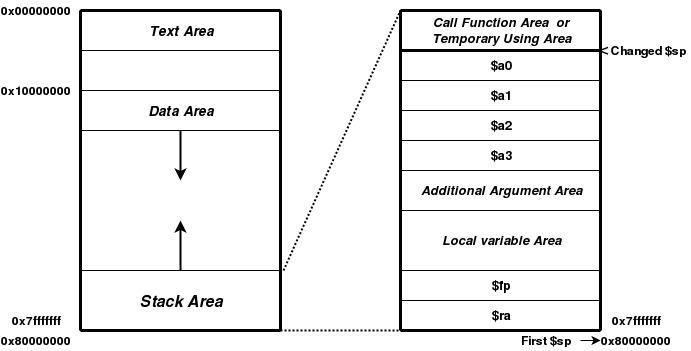
\includegraphics[bb=0 0 691 351,width=100mm]{memory.jpg}
 \end{center}
 \caption{メモリの構成}
 \label{fig:one}
\end{figure}

図1から読み取れるように,メモリはテキスト部,データ部,スタック部の3つで構成している.\verb|0x80000000|から\verb|0xffffffff|までの
アドレスはカーネルエリアとするため,本来アクセスはしない.main関数に渡した引数を保存したり,ロードする場合にのみアクセスする.

また,図にある上下の矢印はデータ領域,スタック領域が広がっていく方向を示している.
静的な領域を確保する場合は,スタック部から,動的な領域を確保する場合は,データ部からそれぞれ領域を伸ばしていく.

スタック部の詳細は図の右側に示す.スタックは関数が呼び出された時に確保され,最小を24バイトとし,以降は倍語長が確保されるように,
8バイト単位でスタックの確保量が変動する.関数中で宣言されたローカル変数は,図の``Local variable Area''に格納される.
また,``Addtional Argument Area''は関数呼び出し時に引数が5つ以上だった場合に確保され,使用される領域である.
そのため,引数が4つ以下の場合はこの領域のサイズは0となる.
この部分に順に引数を並べることで被呼び出し側の関数は引数を順番通りにスタックに格納したり,取り出すことができる.

\$a0から\$a3の4つのレジスタが格納される領域は常に確保されるようにしている.このため,必ず格納される\$raと\$fpの8バイトを
合計した24バイトが最小スタックフレームサイズとなっている.

\$a0より上の領域は,被呼び出し関数の使用領域である.しかし,関数を呼び出すまでは使用されないため,算術式の
計算結果を一時的に格納する場所として利用する.この仕様のため,被呼び出し関数は,自身の変数領域にノイズが残ることがあるため,
変数の初期化が必要となる.しかし,今回は言語定義に初期化が定義されていないため,プログラムを作成する際には,必ず値を代入した
変数を使用することとなる.

\subsection{構文解析時にすること}
\subsubsection{記号表の作成}
コンパイラがコードを生成する中で,変数の情報を管理するためには記号表を用いるのがよい.
これは,変数宣言時や,変数の参照の際に,名前が重複していないか,参照の際に変数がどちらの型であるか,
確保するスタック領域のサイズはいくつかなどを確認するために使用する.

今回はリスト構造を用いて作成した.以下はその変数表構造体Symbolsのメンバである.
\begin{itemize}
\item int          symno          $<$ 変数の番号(Unique)
\item char         *symbolname    $<$ 変数の名前
\item Stype        type           $<$ 変数のタイプ(変数か引数かあるいは関数か)
\item unsigned int size1          $<$ 配列の場合,一次元のサイズ
\item unsigned int size2          $<$ 配列の場合,二次元のサイズ
\item unsigned int address        $<$ 配列の場合,先頭アドレス
\item struct symbols *next        $<$ 大域変数であれば,次は大域変数,局所変数であれば,同様である.
\item struct symbols *branch      $<$ 関数である場合,この先が局所変数となる.
\end{itemize}

コード生成に取り組む上で段々と拡張したため,一つのメンバが複数の役割を果たしていることがある.
そのため,拡張性の面から見るとあまり良くない構造体となっている.

抽象構文木を作成する上で作成したノード構造体Node内にしか含まれない情報もあり,
コード生成に当たり,二つの構造体を対応させながらデータを取得する必要があり,複雑な動きと
なっているため,可読性の観点からもよいとは言えない.今回は作成しなおす時間がなかったため,
そのままとなっている.


\subsection{抽象構文木の各ノードに対応するコードの出力}
\subsubsection{変数領域の確保}
今回作成した言語定義では,受理する変数には大域変数と局所変数の2種類が存在する.今回作成したコンパイラでは,
大域変数はメモリのデータ部に,局所変数はメモリのスタック部に格納される.今回は関数呼び出しへの対応を視野に入れて局所変数を軸に
コード生成に取り組んだため,大域変数に対する挙動メモリの割り当て以外作成できていない.そのため,今回コード生成するプログラムでは,変数は
局所変数のみとする.以下では,変数へのメモリ割り当てを説明する.

大域変数の場合は,配列であるかいなかで挙動が変わる.配列である場合,配列のサイズを要素数を掛けることで算出する.その求めた要素数の積に4バイトを
掛けた値を用いて,アセンブラ指令の\verb|.space|を用いてメモリを割り当てる.配列ではない場合,個別にアセンブラ指令の\verb|.word|を
用いてメモリ割り当てを行う.メモリの値を取り出すには,li命令を用いてアドレスをレジスタに格納した後,lw命令を用いてデータを取り出す.

局所変数の場合は,関数呼び出し時に確保された領域に宣言された順にメモリのアドレスが割り振られる.配列の場合は,4バイト境界で,配列の要素数の
積の分確保される.配列の格納方式には列優先方式を採用した.また,データの取り出しの際は,\$fpから記号表を用いてアドレスを算出し,
lw命令を用いることでデータを取り出すことができる.データを格納する場合は,逆の手順となる.

\subsubsection{算術式}
算術式のコード生成の実現法には,スタックを用いる方法と4つ組中間表現を用いる方法の2通りの方法がある.
スタックを用いる方法は,抽象構文木から直接コードへ変換する方法であり,4つ組中間表現を用いる方法は抽象構文木から4つ組中間表現,
コードの順に変換する.4つ組中間表現には最適化に適しているという利点があるが,スタックを用いた方法の方が実装が用意であったため,
今回はスタックを用いた方法を採用した.

図1での,被呼び出し関数の領域を一時保存領域として利用することでスタックを用いた算術式を実現している.
プッシュ,ポップ操作をコンパイラプログラム中に大域変数として\verb|stack_size|を定義し,\$fpから$-4*stack\_size$した
部分に中間データを格納することで実現している.
4.3.2項でも述べたが,この方式はメモリアクセスが増えるため性能が悪くなる.しかし,実装のしやすさと時間的都合からこちらを選択している.

\subsubsection{代入文}
代入文はまず左辺の変数のアドレスを得る作業を行い,その後,代入する式の部分の計算を行う.算術式と同様に,左辺の変数のアドレスはスタック領域に
一時退避させておく.これは式が代入する式が複雑なものであった場合,上書きされてしまうからである.

両辺のどちらかでも配列が含まれる場合は挙動が少し複雑になる.配列の場合の処理は,配列の変数名をもとに記号表からアドレスを取り出す.
このアドレスは配列の先頭アドレスであるため,このアドレスからのオフセットを計算する必要がある.ここでのオフセットとは配列の要素に
割り当てられた値のことである.割り当てられた値が即値の場合,変数の場合,配列の場合でそれぞれ動作が分岐するので余計に複雑となる.

大域変数の場合は名前からアドレスの取得が容易であるため,比較的実装が簡単である.li命令でアドレスを読み込み,オフセットを算出後,
sw命令を行えば代入文を実現することができる.

\subsubsection{条件分岐}
条件分岐は3部分からなる.式の条件判定,文集合,後続の条件節である.この内,文集合の後と,後続の条件節の末尾にジャンプ先となる
ラベルが必要となる.式の条件判定が真ならば文集合を実行し,偽ならば後続の条件節へと続いていく.また文集合を実行した場合は
後続の条件節をスキップして末尾にジャンプする必要がある.またラベルが重複するとアセンブラ・シュミレータがエラーを出すため,
ラベルは重複しないようにユニークな値としなければならない.

\subsubsection{ループ文}
ループ文にはwhile文とfor文の二種類がある.どちらも条件分岐と似たように式の条件判定部と文集合部からなる.
同様にジャンプ先のラベルを適切に配置することでコード生成を行うことができる.
ループ文には一つのループに三つのラベルが必要となる.先頭と条件部とループ文の外の3箇所である.

ループ文は部分の順番を入れ替えることでコードの実行数を減らすことができる.
while文を例に挙げると,まず条件式の部分にジャンプし,その後真ならば文集合にジャンプし,偽ならそのまま抜けるという順番である.
これにより条件が偽になった場合のジャンプ命令を省略することができる.

またbreak文を実装する上では,ラベル名を分けることはできない.これはbreak文が一つのループを抜けるという特性をもつため,
ラベル名を分けているとループの種類が増えることとなり,break文の実行時に判定処理が必要となる.実装が困難となるため,
while文とfor文のループラベルをユニークにするための大域変数は共通としておく.

\subsubsection{関数呼び出し}
関数呼び出しでは,特に配列の取扱いに関して注意する必要がある.関数で配列を渡す場合,スタックを上手く利用すればまるごと
引き渡すことも不可能ではないが,メモリ効率面からみてもあまり良い選択肢ではない.そのため,通常引数としての配列は先頭アドレスを
渡すこととなる.これは関数呼び出しが一重の場合は問題とならないが,二重,あるいは再帰的な呼び出しをする際には,処理を工夫しなければ
元の配列の先頭アドレスから,アドレスが格納されている\$aレジスタのアドレスに置き換わってしまう.今回の実験ではこの処理が
解決できず,関数を複数回呼び出したときのコード生成ができなかった.



%%%%%%%%%%%%%%%%%%%%%%%%%%%%%%%%%%%%%%%%%%%%%%%%%%%%%%%%%%%%%%%%
\section{コンパイラ作成過程で工夫した点}
%%%%%%%%%%%%%%%%%%%%%%%%%%%%%%%%%%%%%%%%%%%%%%%%%%%%%%%%%%%%%%%%
本実験におけるコンパイラ作成過程で工夫した点の一つはスタックを利用した局所変数の格納である.
図1のような形をプロットとし,記号表と対応させたアドレスを用いることで実現することができた.
これにより関数呼び出しの際に,引数をスタックフレームに格納するだけで受け渡しができるようになった.
実装はしなかったが,return文の実装も容易である.レジスタへの影響が小さいのであまり意識することなく
レジスタを使用することができる.このスタックフレームを作成する過程で気づいたが,スタックフレーム長を
調整することで返り値を複数可させることも可能であるように感じた.
関数呼び出しの後,返り値用のスタック領域を確保しておくことで,2つ目,3つ目の返り値が実現できる.

また,今回は抽象構文木を作成していることから処理が段階的に実施される.そのため,
各処理にデバッグ用の出力コードを埋め込み,\verb|#ifdef|を利用することでデバックの切り替えをできるように
工夫を行った.これによりアセンブラ出力時の関数の動きがわかりやすくなり,
MAPSに通したいときには,コメントアウト一つで余分な出力が消え,シュミレートを行うことができた.
これによりいくつかバグを発見することができた.このことから,デバックの大切さを再認識した.

また,抽象構文木生成関数において任意の子をもつノードを生成する\verb|make_nchile_node|関数を実装した.
これは,第二引数のノードを親として,それ以降の引数のノードを子とする関数である.
これによりノードを作成する関数の省略に成功した.

%%%%%%%%%%%%%%%%%%%%%%%%%%%%%%%%%%%%%%%%%%%%%%%%%%%%%%%%%%%%%%%%
\section{最終課題を解くために(定義した言語で)書いたプログラムの概要}
%%%%%%%%%%%%%%%%%%%%%%%%%%%%%%%%%%%%%%%%%%%%%%%%%%%%%%%%%%%%%%%%
\subsection{yaccプログラム: langspec.y}
##
\subsubsection{定義部}
プログラム中で登場する終端記号および非終端記号の型が定義されている.
主にノードかオペランドかの二種類となる.
\subsubsection{規則部}
通常の書き方に応じて記述を行った.数値に関してはlexレベルでは記号に未対応とさせ,
yaccレベルで対応させている.これにより,配列の中で式が要素として与えられた際に,
オペランド同士の隙間がなくても読み取ることができる.
\subsubsection{ユーザ定義サブルーチン部}
ここでは入力されたテキストを読み込んで,それが規則部で記述したとおりに構文が構成され
ているかを調べ,エラーが生じたら途中でエラー出力とともにプログラムを終了し,
エラーがなければ抽象構文木生成,シンボルテーブルの表示,コード生成を行う.
いつも抽象構文木とシンボルテーブルの表示が行われると不便であるため,
コマンドライン引数としてなんらかの引数を渡した場合のみ実行されるように改良した.
そのため,引数になにも与えずにプログラムを実行すると,コード生成のみが行われる.
##
\subsection{lexプログラム: langspec.l}
##
\subsubsection{定義部}
使用するヘッダファイルを記述している.抽象構文木作成のための関数を字句解析レベルで
使用するため,``ast.h''も含まれている.
\subsubsection{規則部}
入力文字列に対して,適切な終端記号を返す.また関数の局所変数テーブルを作成するために,
この段階で記号表のルート部分をこの段階で作成している.また数値に関しては,
字句解析段階で数値ノードとして作成する.
\subsubsection{ユーザ定義サブルーチン部}
lexレベルでは何もしない.
##
\subsection{抽象構文木作成およびコード生成プログラム: ast.c}
##
\subsubsection{抽象構文木生成プログラム}
以下の関数を用いて抽象構文木を生成し,出力する.
各プログラムに関して,それぞれ簡単な説明を行う.
\begin{itemize}
\item \verb|make_num_node|
\begin{itemize}
数字ノードを作成する.返り値はNode*型.Node型に関する説明はヘッダファイルの部分で行う.
Node型のメンバvalueに整数値を格納して返す.
\end{itemize}
\item \verb|make_ident_node|
\begin{itemize}
識別子ノードを作成する.識別子ノードに該当するのは関数や変数,配列などである.
Node型のメンバvalueにユニークなシンボルナンバーを格納して返す.
\end{itemize}
\item \verb|make_new_ident_node|
\begin{itemize}
配列の宣言時に使用.機能は\verb|make_ident_node|と変わらないが,
配列宣言用に改造されている.
\end{itemize}
\item \verb|make_nchild_node|
\begin{itemize}
ノードの子ノードを生成する際に使用.第2引数のノードを親とし,以降の引数のノードを
子とする.
\end{itemize}
\item \verb|get_child_num|
\begin{itemize}
ノードタイプによる子の数を取得する.
\end{itemize}
\item \verb|sym_lookup|
\begin{itemize}
名前から識別子のシンボルナンバーを取得する.
\end{itemize}
\item \verb|sym_add|
\begin{itemize}
記号表に識別子を加える関数である.
\end{itemize}
\item \verb|sym_lookup_name|
\begin{itemize}
識別子のシンボルナンバーから識別子の名前を取得する.
\end{itemize}
\item \verb|sym_lookup_entry|
\begin{itemize}
関数の局所変数テーブルの先頭を取得するために使用する.
\end{itemize}
\item \verb|get_ntype_name|
\begin{itemize}
構文木出力でしようする.ノードのタイプから名前を返す.
\end{itemize}
\item \verb|print_ast_tree|
\begin{itemize}
作成されたノード集合から構文木を出力する.
\end{itemize}
\item \verb|print_symbol_table|
\begin{itemize}
作成された記号表を出力する.それぞれの記号のシンボルナンバーも同時に出力する.
\end{itemize}
\end{itemize}
##
\subsubsection{コード生成プログラム}
以下の関数を用いてコード生成し,出力する.
各プログラムに関して,それぞれ簡単な説明を行う.
\item \verb|calc_arg_node_depth|
\begin{itemize}
関数の引数の数を取得する.
\end{itemize}
\item \verb|generate_program_code|
\begin{itemize}
コード生成の開始関数.この関数から順にコード生成関数を呼び出していく.
\end{itemize}
\item \verb|generate_initial_code|
\begin{itemize}
コード生成にあたり,最初に書くべきコードを生成する.
\end{itemize}
\item \verb|generate_function_list_code|
\begin{itemize}
関数の数だけ関数のコード生成を行う.
\end{itemize}
\item \verb|generate_function_code|
\begin{itemize}
関数に対応するコード生成を行う.開始処理,メイン処理,終了処理の3部分で構成される.
\end{itemize}
\item \verb|calc_local_variable_size|
\begin{itemize}
関数における局所変数領域のサイズを計算する関数.スタックの確保に使用する.
\end{itemize}
\item \verb|generate_gloval_variables_definitions|
\begin{itemize}
大域変数の宣言に関するコードを生成する.
\end{itemize}
\item \verb|generate_statement_code|
\begin{itemize}
文に対応するそれぞれの関数を呼び出す.
\end{itemize}
\item \verb|generate_assign_code|
\begin{itemize}
代入文に対応するコードを生成する.
\end{itemize}
\item \verb|generate_arithmetic_code|
\begin{itemize}
算術式に対応するコードを生成する.
\end{itemize}
\item \verb|set_ident_address|
\begin{itemize}
変数や配列にアドレスを割り当てる.
\end{itemize}
\item \verb|get_ident_address|
\begin{itemize}
変数のアドレスを取得する.
\end{itemize}
\item \verb|get_array_address|
\begin{itemize}
配列のアドレスを取得する.
\end{itemize}
\item \verb|generate_while_code|
\begin{itemize}
while文に対応するコードを生成する.
\end{itemize}
\item \verb|generate_expression_code|
\begin{itemize}
ループ文や条件分岐における式評価を行うコードを生成する.
\end{itemize}
\item \verb|generate_if_code|
\begin{itemize}
if文に対応するコードを生成する.
\end{itemize}
\item \verb|generate_for_code|
\begin{itemize}
for文に対応するコードを生成する.
\end{itemize}
\item \verb|generate_funccall_code|
\begin{itemize}
関数呼び出しに対応するコードを生成する.
\end{itemize}

\begin{itemize}
\end{itemize}
\end{itemize}
##
\subsection{ast.c のヘッダ: ast.h}
##
抽象構文木やコード生成で用いる列挙型や構造体の定義や,関数のプロトタイプ宣言が記述してある.
作成したが使用していないものもそのまま残してある.例えば,構造体の``Fours'' は四つ組中間表現の
実装に向けて使用する予定だったが,スタック方式を採用したため,使用していない.

またここで構造体Nodeの説明を行う.これは抽象構文木におけるノードを表す構造体である.
メンバは以下のとおりである.
\begin{itemize}
\item  Ntype type
\item  int value 
\item  int value2
\item  char *name
\item  int n\_child
\item  struct node **child
\end{itemize}
typeにはノードの種類が,valueにはノードに対応する値が格納され,識別子などの場合は
nameに変数名,関数名などが格納される.n\_childは子の数であり,childは子ノードへの
アクセスに利用する.


##
%%%%%%%%%%%%%%%%%%%%%%%%%%%%%%%%%%%%%%%%%%%%%%%%%%%%%%%%%%%%%%%
\section{最終課題の実行結果}
%%%%%%%%%%%%%%%%%%%%%%%%%%%%%%%%%%%%%%%%%%%%%%%%%%%%%%%%%%%%%%%%
最終課題は1から6を行ったが,6に関しては関数の再帰呼び出しに不具合があり,上手くいかなかった.
代わりに別の関数の呼び出しを行うプログラムを作成し,単純な関数呼び出しは実装できたことが確認できた.
以降に実行結果として,各最終課題のアセンブリコード実行後のメモリの状態を記載する.
\subsection{最終課題1}
ステップ数: 391 
\begin{verbatim}
# tag=2047 index=255
7fffffd0: 00000000 00000000 00000001 0000000a
7ffffff0: 0000000b 00000037 00000000 00000018
###
# tag=2048 index=0
###
\end{verbatim}
\subsection{最終課題2}
ステップ数: 221 
\begin{verbatim}
# tag=2047 index=255
7fffffd0: 00000000 00000000 00000001 00000005
7ffffff0: 00000006 00000078 00000000 00000018
###
# tag=2048 index=0
###
\end{verbatim}
\subsection{最終課題3}
ステップ数: 3249 
\begin{verbatim}
# tag=2047 index=255
7fffffc0: 00000000 00000000 00000001 0000001e
7fffffe0: 00000008 00000004 00000002 00000010
7ffffff0: 0000001f 00000000 00000000 00000018
###
# tag=2048 index=0
###
\end{verbatim}
\subsection{最終課題3改良}
ステップ数: 2301
\begin{verbatim}
# tag=2047 index=255
7fffffc0: 00000000 00000000 00000001 0000001e
7fffffe0: 00000008 00000004 00000002 00000010
7ffffff0: 0000001f 00000000 00000000 00000018
###
# tag=2048 index=0
###

\end{verbatim}
\subsection{最終課題4}
ステップ数: 391502
長いため,0から50までとする.
\begin{verbatim}
# tag=2047 index=255
7ffff020: 00000000 00000000 00000002 7ffff050
7ffff040: 000003e8 000001f5 00000003 000003e8
7ffff050: 00000100 00000002 00000002 00000002
7ffff060: 00000001 00000002 00000001 00000002
7ffff070: 00000001 00000001 00000001 00000002
7ffff080: 00000001 00000002 00000001 00000001
7ffff090: 00000001 00000002 00000001 00000002
7ffff0a0: 00000001 00000001 00000001 00000002
7ffff0b0: 00000001 00000001 00000001 00000001
7ffff0c0: 00000001 00000002 00000001 00000002
7ffff0d0: 00000001 00000001 00000001 00000001
7ffff0e0: 00000001 00000002 00000001 00000001
7ffff0f0: 00000001 00000002 00000001 00000002
7ffff100: 00000001 00000001 00000001 00000002

\end{verbatim}
\subsection{最終課題5}
ステップ数: 1652 
\begin{verbatim}
# tag=2047 index=255
7fffff90: 00000000 00000000 00000000 00000008
7fffffa0: 00000020 00000001 00000000 00000000
7fffffb0: 00000000 00000000 00000001 00000002
7fffffc0: 00000003 00000004 00000005 00000006
7fffffd0: 00000007 00000008 00000013 00000016
7fffffe0: 0000002b 00000032 00000002 00000002
7ffffff0: 00000002 00000000 00000000 00000018
###

\end{verbatim}
\subsection{最終課題6}
ステップ数: 4696
\begin{verbatim}
7fffffc0: 00000003 00000000 0000000a 00000000
7fffffd0: 00000004 00000002 00000009 00000007
7fffffe0: 7fffffd0 00000005 00000009 0000000a
7ffffff0: 00000001 00000008 00000000 00000018
###
\end{verbatim}
\subsection{成功した関数呼び出しプログラム}
ステップ数: 2301
\begin{verbatim}
# tag=2047 index=255
7fffffa0: 00000000 00000000 00000002 00000003
7fffffc0: 00000005 00000000 7fffffd0 000012dc
7fffffd0: 7fffffe0 7fffffec 00000000 00000000
7fffffe0: 00000003 00000002 00000001 00000003
7ffffff0: 00000002 00000000 00000000 00000018
###

\end{verbatim}
%%%%%%%%%%%%%%%%%%%%%%%%%%%%%%%%%%%%%%%%%%%%%%%%%%%%%%%%%%%%%%%
\section{考察}
%%%%%%%%%%%%%%%%%%%%%%%%%%%%%%%%%%%%%%%%%%%%%%%%%%%%%%%%%%%%%%%%
ステップ数からわかるように実行命令数が多い.これは値を取り出す一つ一つにスタックの出し入れ操作が含まれているから
である.また,最終課題3の改良前と改良後でステップ数が3分の1程減少している.これは算術式の中に現れる変数や定数項の数が減ったためである.
このことから,一つの演算子や項に対するステップ数の依存度の高さが読み取れる.そのため,最適化や適切なレジスタ操作を
行わない,性能の低いコンパイラによって生成されたプログラムのコードはステップ数が増え,性能が悪化することが分かる.

##
作成過程で気づいたこともいくつか存在する。C言語においては関数の順番は使用する順に定義する
必要がある。順番を気にせずにプログラムの作成を行うにはプロトタイプ宣言が必要となる。
これは関数のスタックエリア確保の際に,スタックサイズを計算するために,関数の引数の
種類と数が必要になるためであると考えることができる. 呼び出し側関数のスタックを確保する
際に,関数中に登場する関数呼び出しで呼ばれる関数の引数が4つ以上の場合,新たにスタックエリア
を確保しなければならない(図1でのAdditional Stack Area). 

また,MIPS規約に存在する倍語長境界を維持するというルールであるが,これは倍語長を
扱う際に,実装上最大のデータ単位で考えることで,データ型の違いによるスタック確保
の処理の違いを吸収する意味があるのではないかと考えた. そのため,あらゆるデータを32bit
単位で扱う今回のコンパイラではあまり意味のないルールとなっているのではないかと考えられる.

##
%%%%%%%%%%%%%%%%%%%%%%%%%%%%%%%%%%%%%%%%%%%%%%%%%%%%%%%%%%%%%%%%
\section{ソースプログラムのある場所}
%%%%%%%%%%%%%%%%%%%%%%%%%%%%%%%%%%%%%%%%%%%%%%%%%%%%%%%%%%%%%%%%

作成したソースプログラ以下の場所に保存してある.
一つ目はレポートに向けて途中で切り上げたコンパイラである.
二つ目は最終課題6のコード生成に向けて改良を加え続けているものである.
/home/users/ecs/09428526/git/C-exp/compiler/personal/ptype2

/home/users/ecs/09428526/git/C-exp/compiler/personal/sample

##
ファイルはそれぞれ以下に対応する
\begin{itemize}
\item yacc: langspec.y
\item tex: langspec.l
\item 抽象構文木作成プログラム: ast.c
\item 抽象構文木ヘッダファイル: ast.h
\end{itemize}
%%%%%%%%%%%%%%%%%%%%%%%%%%%%%%%%%%%%%%%%%%%%%%%%%%%%%%%%%%%%%%%%
\section{最終課題およびコード生成に成功したプログラム}
%%%%%%%%%%%%%%%%%%%%%%%%%%%%%%%%%%%%%%%%%%%%%%%%%%%%%%%%%%%%%%%%
\subsection{最終課題1}
{\fontsize{10pt}{11pt} \selectfont
\begin{verbatim}
     1	func main(){
     2	 define i; 
     3	 define sum;
     4	
     5	 sum = 0;
     6	 i = 1;
     7	 while(i < 11) {
     8	    sum = sum + i;
     9	    i = i + 1;
    10	 }
    11	}
\end{verbatim}
}
\subsection{最終課題2}
{\fontsize{10pt}{11pt} \selectfont
\begin{verbatim}
     1	func main(){
     2	  define i;
     3	  define fact;
     4	  
     5	  fact = 1;
     6	  i = 1;
     7	  while(i < 6) {
     8	    fact = fact * i;
     9	    i = i + 1;
    10	  }
    11	}
\end{verbatim}
}
\subsection{最終課題3}
{\fontsize{10pt}{11pt} \selectfont
\begin{verbatim}
     1	func main(){
     2	  define fizz;
     3	  define buzz;
     4	  define fizzbuzz;
     5	  define others;
     6	  define i;
     7	  
     8	  fizz = 0; 
     9	  buzz = 0;
    10	  fizzbuzz = 0; 
    11	  others = 0;
    12	  i = 1;
    13	  while(i < 31){
    14	    if ((i / 15) * 15 == i)
    15	      fizzbuzz = fizzbuzz + 1;
    16	    else if ((i / 3) * 3 == i){
    17	      fizz = fizz + 1;
    18	    }
    19	    else if ((i / 5) * 5 == i){
    20	      buzz = buzz + 1;
    21	    }else{
    22	      others = others + 1;
    23	    }
    24	
    25	    i = i + 1;
    26	  }
    27	}b
\end{verbatim}
}
\subsection{最終課題3(改良)}
{\fontsize{10pt}{11pt} \selectfont
\begin{verbatim}
     1	func main(){
     2	  define fizz;
     3	  define buzz;
     4	  define fizzbuzz;
     5	  define others;
     6	  define i;
     7	  
     8	  fizz = 0; 
     9	  buzz = 0;
    10	  fizzbuzz = 0; 
    11	  others = 0;
    12	  i = 1;
    13	  while(i < 31){
    14	    if (i%15 == 0)
    15	      fizzbuzz = fizzbuzz + 1;
    16	    else if (i%3 == 0){
    17	      fizz = fizz + 1;
    18	    }
    19	    else if (i%5 == 0){
    20	      buzz = buzz + 1;
    21	    }else{
    22	      others = others + 1;
    23	    }
    24	
    25	    i++;
    26	  }
    27	}
\end{verbatim}
}
\subsection{最終課題4}
{\fontsize{10pt}{11pt} \selectfont
\begin{verbatim}
     1	func main(){
     2	  define N;
     3	  define i;
     4	  define j;
     5	  define k;
     6	  array a[1001];
     7	 
     8	  N = 1000;
     9	  i = 1;
    10	  while (i <= N) {
    11	    a[i] = 2;
    12	    i = i + 1;
    13	  }
    14	  
    15	  i = 2;
    16	  while( i <= N/2) {
    17	    j = 2;
    18	    while(j <= N/i){
    19	     k = i * j;
    20	     a[k] = 1;             	       
    21	     j = j + 1;
    22	    }
    23	    i = i + 1;
    24	  }
    25	  a[0] = 256;
    26	}
\end{verbatim}
}
\subsection{最終課題5}
{\fontsize{10pt}{11pt} \selectfont
\begin{verbatim}
     1	func main(){
     2	  array matrix1[2][2];
     3	  array matrix2[2][2];
     4	  array matrix3[2][2];
     5	  
     6	  define i;
     7	  define j;
     8	  define k;
     9	  
    10	  matrix1[0][0] = 1;
    11	  matrix1[0][1] = 2;
    12	  matrix1[1][0] = 3;
    13	  matrix1[1][1] = 4;
    14	  
    15	  matrix2[0][0] = 5;
    16	  matrix2[0][1] = 6;
    17	  matrix2[1][0] = 7;
    18	  matrix2[1][1] = 8;
    19	  
    20	  for(i=0;i<2;i++){
    21	    for(j=0;j<2;j++){
    22	      matrix3[i][j] = 0;
    23	    }
    24	  }
    25	  
    26	  for(i=0;i<2;i++){
    27	    for(j=0;j<2;j++){
    28	      for(k=0;k<2;k++){
    29		matrix3[i][j] = matrix3[i][j] + matrix1[i][k] * matrix2[k][j];
    30	      }
    31	    }
    32	  }
    33	}
\end{verbatim}
}
\subsection{最終課題6}
{\fontsize{10pt}{11pt} \selectfont
\begin{verbatim}
     1	func quicksort(array a[], define l, define r){
     2	    define v, i, j, t;
     3	    define ii;
     4	
     5	    if (r > l){
     6		v = a[r]; i = l - 1; j = r;
     7		for(;;){
     8		    while(a[++i] < v) ;
     9		    while(a[--j] > v);
    10		    if (i >= j) break;
    11		    t = a[i]; a[i] = a[j]; a[j] = t;
    12		}	
    13	    t = a[i]; a[i] = a[r]; a[r] = t;
    14	
    15	    funccall quicksort(a, l, i-1);
    16	    funccall quicksort(a, i+1, r);
    17	    }
    18	}
    19	
    20	func main(){
    21	    array data[10];
    22	    data[0] = 10;
    23	    data[1] = 4;
    24	    data[2] = 2;
    25	    data[3] = 7;
    26	    data[4] = 3;
    27	    data[5] = 5;
    28	    data[6] = 9;
    29	    data[7] = 10;
    30	    data[8] = 1;
    31	    data[9] = 8;
    32	
    33	    funccall quicksort(data, 0, 9);
    34	}
\end{verbatim}
}
\subsection{成功した関数呼び出しプログラム}
{\fontsize{10pt}{11pt} \selectfont
\begin{verbatim}
     1	func tmp(array a[], array b[]){
     2	     define d;
     3	     b[0] = a[0];
     4	     b[1] = a[1];
     5	     d = b[0]+b[1];
     6	
     7	}
     8	
     9	func main(){
    10	     array a[3];
    11	     array b[2];
    12	     a[0] = 3;
    13	     a[1] = 2;
    14	     a[2] = 1;
    15	     b[0] = 0;
    16	     b[1] = 0;
    17	     funccall tmp(a,b);
    18	}
\end{verbatim}
}
\end{document}
